\subsection{Abstract}
The position and number of functional groups of pyridin-4-ylethynyl functionalized pyrene molecules control their self-assembly and electronic properties. To access these in UHV, decoupling of the underlying substrate (Cu(111)) is mandatory and achieved here with a \textit{h}-BN spacer layer. As a result unperturbed HOMO and LUMO states are resolved in STM. While STS shows a band gap that decreases with increasing number of functional groups, it is not affected by their position and the molecular assembly observed STM. The gap between pronounced HOMO/LUMO states is modulated by the electronically corrugated \textit{h}-BN/Cu(111) interface and predominantly determined by the larger shift of the LUMO states. UV/Vis measurements in solution reveal a high quantum yield of the fluorescence emission at wavelengths consistent with ab-initio DFT calculations. Finally, the ability of trans-pyrene to act as host system for cis-pyrene is shown.

\subsection{Introduction}
Pyrene’s optical properties\cite{Figueira-Duarte_Pyrene_2011} make it a promising candidate for potential applications. 1,3,6,8-tetrasubstituted pyrenes are used in a variety of applications, including blue\cite{Moorthy_Steric_2007,Sonar_pyrenes_2010,Feng_Pyrene_2012}, yellow\cite{Sonar_pyrenes_2010}, green\cite{Chang_efficient_2012} and multilayered\cite{Thomas_pyrene_2012} OLEDs. The emergence of these compounds in applications is based on fundamental research in (not only, but including) surface science conducted under conditions where unperturbed photophysical properties of the molecule can be controlled and tuned. Optical properties are often investigated on transparent insulating bulk materials (Differential Reflectance Spectroscopy (DRS) - PTCDA/mica)\cite{Proehl_Formation_2004}, (Reflectance anisotropy spectroscopy - $\alpha$-quaterthiophene/potassium hydrogen phthalate)\cite{Bussetti_reflectance_2009} but are also possible on nontransparent HOPG(photoluminescence - quater – (4T) and sexithiophene (6T) films/HOPG)\cite{Schneider_Morphology_2002} or SiO2 (pentacene, perfluoropentacene, and diindenoperylene/SiO2)\cite{Heinemeyer_Real-Time_2010} surfaces. These space averaging techniques are complemented with measurements on atomic length scales where sub-molecular topographic and electronic structure are investigated by STM and STS in UHV. These need a conducting support for the molecules to adsorb on, making the choice of a suitable substrate important.
Molecules adsorbed on metal surfaces interact with their support, resulting in luminescence quenching (Photoluminescence - Quaterthiophene and PTCDA on Ag(111))\cite{Gebauer_Luminescence_2004} and broadened frontier molecular orbitals. Mediated by the presence of a metal, these exhibit considerable interaction with low-lying orbitals, changing their shape\cite{Chavy_Interpretation_1993}. To minimize the interaction with a metallic substrate, spacer layers of insulating materials are used. 
Recent years of research have increased the variety of these while a continuous decrease in layer thickness could be achieved. For example, ultrathin (~6) layers of NaCl (pentacene/NaCl)\cite{Repp_molecules_2005} and KCl\cite{Koslowski_adsorption_2017} are utilized for direct imaging of unperturbed molecular orbitals in STM. The thinnest spacer (since it consists only of a single layer of atoms) is provided by a \textit{h}-BN monolayer. Its large band gap is used to minimize interaction with the metallic substrate as shown experimentally\cite{joshi_boron_2012} and theoretically (DFT – silicene/\textit{h}-BN/Cu(111))\cite{Kanno_Electronic_2014}. Here self-assembly and electronic properties can be studied in STM/STS and compared with other unperturbed systems as well as with theory. 
In this work we propose functionalized pyrene building-blocks\cite{Casas-Solvas_Synthesis_2014,Feng_Functionalization_2016} for self-assembled regular molecular arrays on surfaces. Functionalization with pyridin-4-ylethynyl\cite{Figueira-Duarte_Pyrene_2011} makes pyrene an versatile agent for controlled self-assembly. Cis- , trans- and tetra functionalized pyridin-4-ylethynyl-pyrene was already investigated on Ag(111) system resulting in one-dimensional coordination chains, two-dimensional arrays and chiral, porous kagom\'e networks, where assembly is controlled by the number and position of substituents.\cite{Kaposi_Supramolecular_2016} 
Hereinafter the influences of self-assembly, leg functionalization\cite{Kurata_donor_2017} and intra moir\'e position\cite{Sushobhan_Control_2014} on the band gap is investigated. Mandatory electronic decoupling is achieved either on \textit{h}-BN/Cu(111) or in solution where the molecules’ density of states is not influenced by a supporting metal.

\subsection{Results}

We investigate three different derivatives of pyridin-4-ylethynyl substituted pyrenes shown in \autoref{fig:pyrene-fig1}: \subref{fig:pyrene-fig1-tetra} Tetra-pyrene has four functional groups added at position 1,4,6 and 8. The point symmetric result is therefore neither chiral nor bears a dipole moment. \subref{fig:pyrene-fig1-trans} Trans-pyrene is substituted at the positions 1 and 6 (“equatorial” positions) resulting in a pro-chiral molecule. \subref{fig:pyrene-fig1-cis} Cis-pyrene is functionalized at longitudinal positions 1 and 8. With both electron rich groups being on the same side, they create a permanent dipole moment of 4.1 D in this non-chiral molecule.

\begin{figure}[b] \centering
\subfigure[]{
		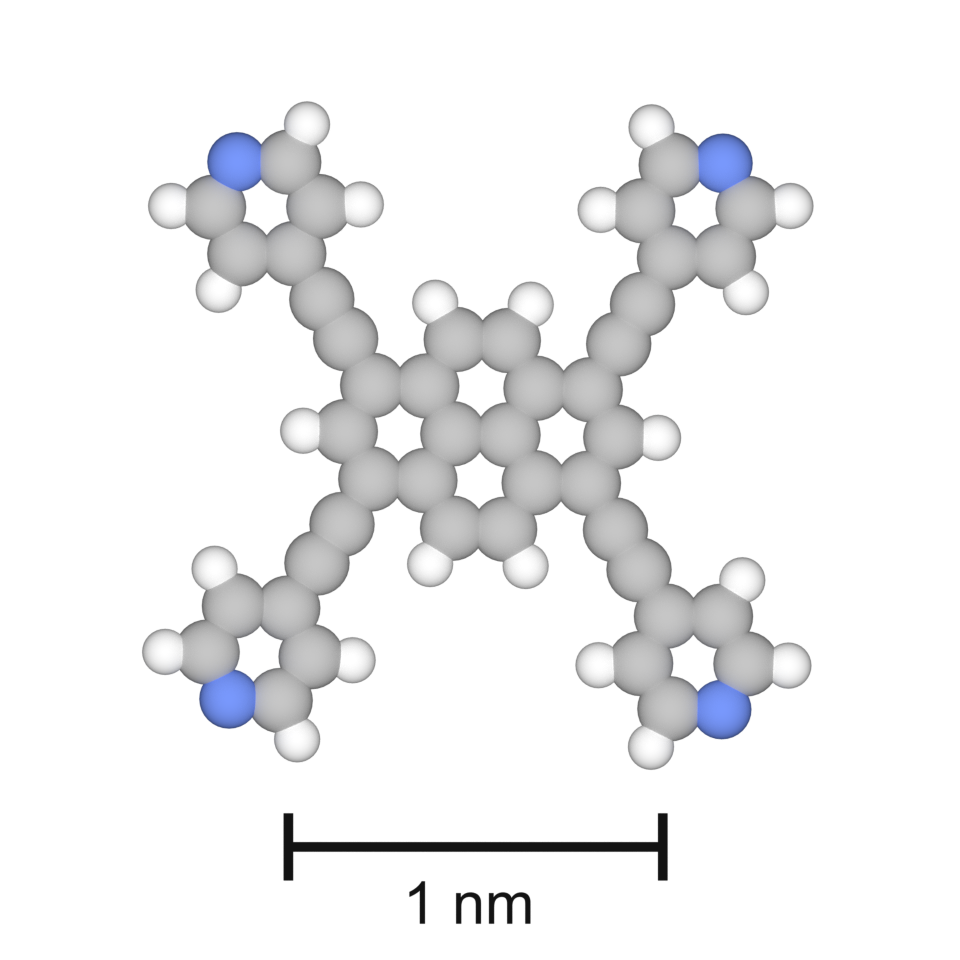
\includegraphics[width=0.25\textwidth]{./images/paper/pyrene/tetra-model}
		\label{fig:pyrene-fig1-tetra}
	}
\subfigure[]{
		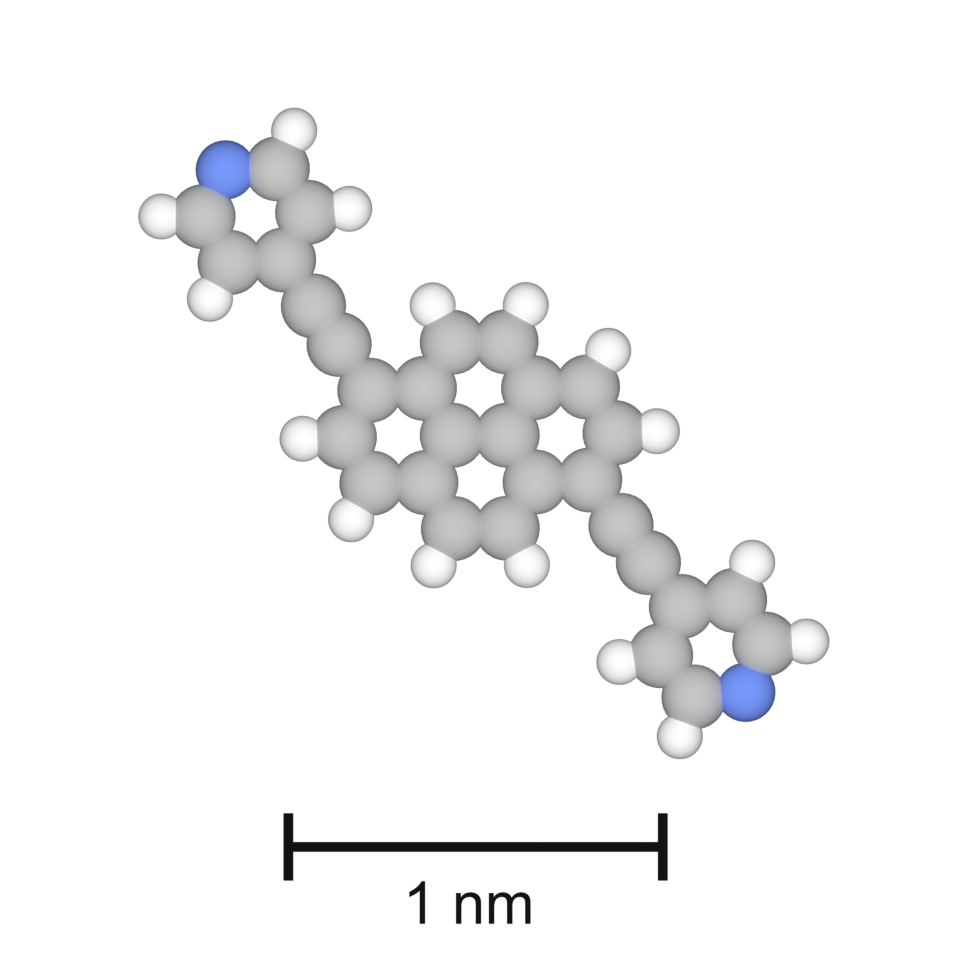
\includegraphics[width=0.25\textwidth]{./images/paper/pyrene/trans-model}
		\label{fig:pyrene-fig1-trans}
	}
\subfigure[]{
		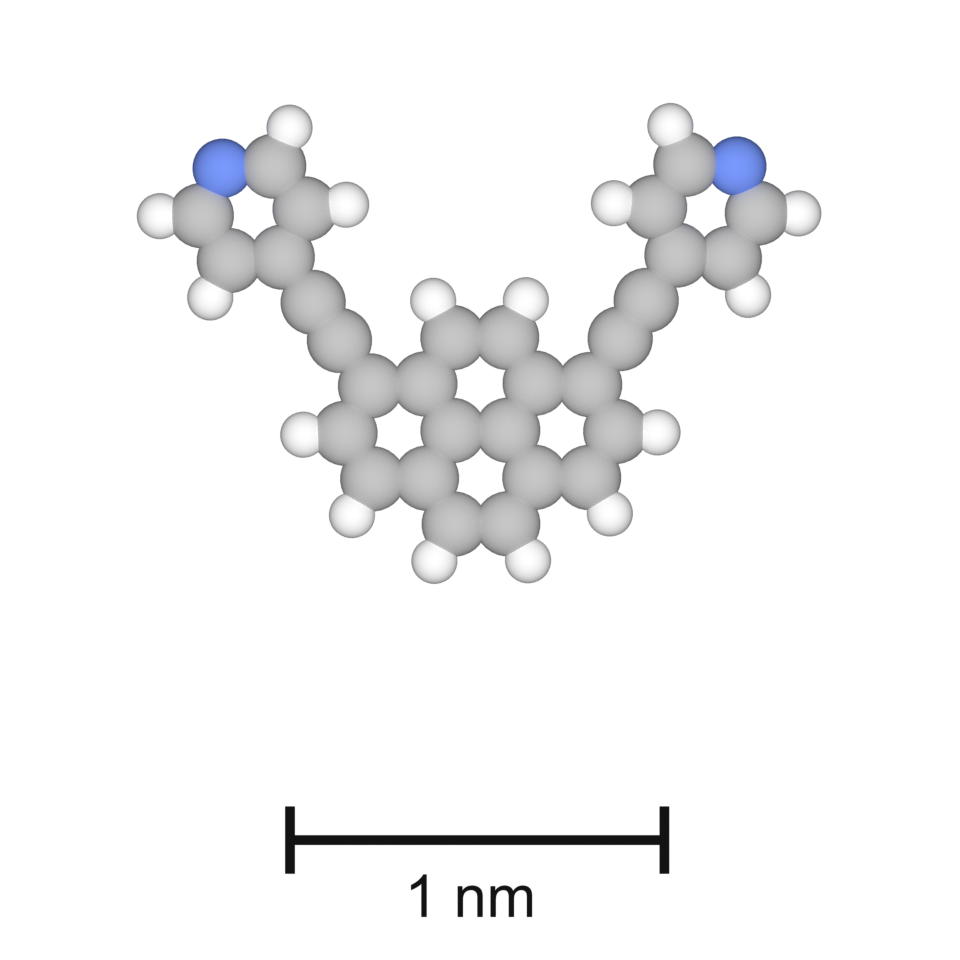
\includegraphics[width=0.25\textwidth]{./images/paper/pyrene/cis-model}
		\label{fig:pyrene-fig1-cis}
	}
	\caption{AM1 relaxed functionalized pyrene species in gas phase. Structure of \subref{fig:pyrene-fig1-tetra} tetra-, \subref{fig:pyrene-fig1-trans} trans- and \subref{fig:pyrene-fig1-cis} cis-pyridil functionalized pyrene molecule. All species are virtually flat.}
	\label{fig:pyrene-fig1}
\end{figure}

The 4-ylethynyl functionalization leads to a certain degree of freedom to rotate the group in plane or tilt the pyridil ring around the C-C bond connecting it to the rigid pyrene core (compare appendix S13).


\begin{figure}[] \centering
	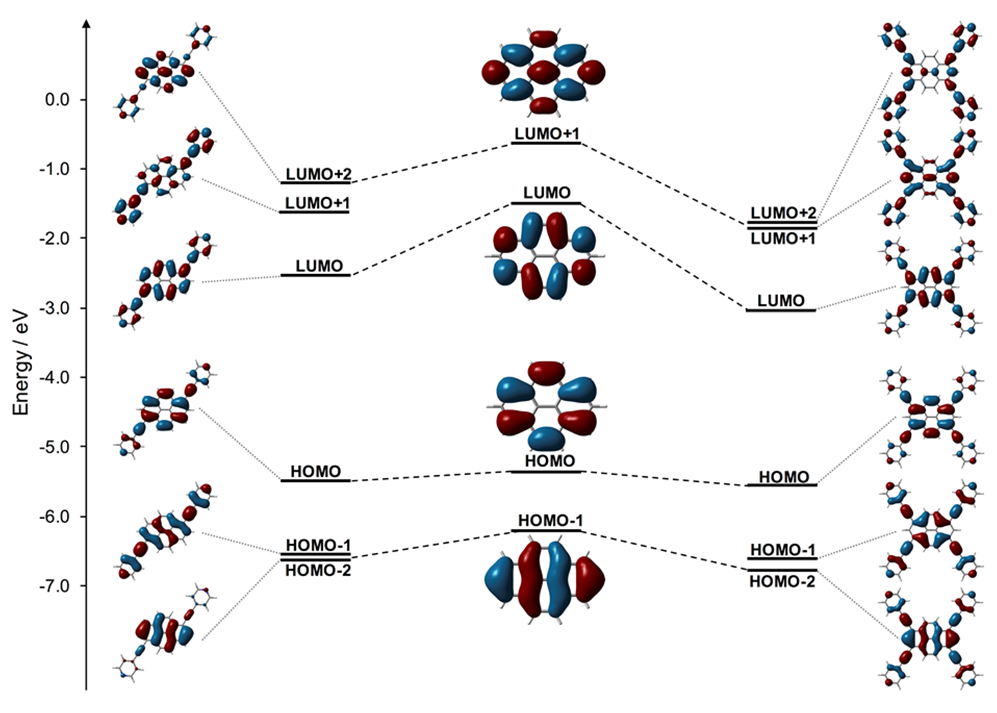
\includegraphics[width=0.7\textwidth]{./images/paper/pyrene/figure-2}
	\caption{Schematic drawing of the frontier Kohn−Sham orbitals for trans- \& tetra-pyridil-ethynyl substituted pyrene derivatives, together with orbital correlation diagram in comparison of the molecular orbitals (MOs) for pyrene itself, at the B3LYP/6-31G** level of DFT.}
	\label{fig:pyrene-fig2}
\end{figure}

To evaluate the effect of the substitution on the pyrene core DFT calculations were performed (B3LYP/6-31G** level of theory, in vacuum). The frontier Kohn-Sham orbitals of pyrene and di- and tetra-substituted pyridylethynyl pyrene are shown in \autoref{fig:pyrene-fig2} and \autoref{fig:pyrene-S4}, \autoref{fig:pyrene-S8}.
These show that pyrenes have large orbital coefficients at the 1-, 3-, 6- and 8-positions, with the nodal plane going through the 2- and 7- positions.\cite{Kurata_donor_2017,Maeda_Alkynylpyrenes_2006,Diring_Luminescent_2009,Crawford_experimental_2011,Ji_Electron_2015,Lee_Enhanced_2012} Consequently, orbital interactions between the pyrene and the pyridylethynyl MOs have an effect on stabilizing the highest occupied (HOMO) and lowest unoccupied (LUMO) molecular orbital energy levels. While the HOMO stabilization plays only a small part, the considerable lowering of the LUMO energy levels lead to smaller HOMO-LUMO gaps. The picture of orbital interactions is similar in cis- and tetra-pyrene, with the HOMO-LUMO gap being influenced mostly by the number of substituents: The gap of tetra-substituted pyrene (\SI{2.54}{\eV}) becomes narrower than that of bi-substituted trans-pyrene (\SI{2.95}{\eV}), which is in accordance to experimental findings (vide infra) and previous literature reports.\cite{Maeda_Alkynylpyrenes_2006, Diring_Luminescent_2009, Lee_Enhanced_2012}
%%%
As both the electronic and optical properties of molecules are quenched or at least altered upon adsorption on metal surfaces it is necessary to decouple the functional pyrenes from the metallic substrate. Therefor we grow a single layer of \textit{h}-BN on a Cu(111) single crystal. Besides its insulating properties we have chosen this lattice mismatched system (\textbf{citation}) to make use of its spatially modulated surface potential (\textbf{citation}). Depending on the registry of adsorbate (B, N) and substrate (Cu) atoms the surface is divided in regions of larger (pore) and lower (wire) work function. This moir\'e is used here to fine tune the energy of molecular states.
When choosing a bias voltage close to the onset of the LUMO one can easily note molecules in the pore region already contributing to the tunneling current resulting in a bright protrusion in STM although \textit{h}-BN/Cu(111) forms a weakly corrugated layer (\textbf{citation}). 

After deposition tetra-pyrene molecules assemble in dense packed islands shown in \autoref{fig:pyrene-fig3}. Every molecule within the island shows the same orientation. The unit cell is triclinic (\SI{1.63}{\nano \meter} $\times$ \SI{1.50}{\nano \meter}, \SI{92}{\degree}) and holds a single molecule. The binding motif is guided by the functional groups where a pyridil ring forms a bond with the adjacent pyridil ring of the neighboring molecule. Assuming flat pyridil groups parallel to the surface, the assembly is characterized by two intermolecular distances $d_1$ and $d_2$ between two pyridil groups, $d_1$ ($d_2$) pointing to the long (short) side of the pyrene core as indicated by black lines connecting neighboring nitrogen and hydrogen termini in the inset of \autoref{fig:pyrene-fig3b}. 

\begin{figure}[] \centering
	\subfigure[]{
		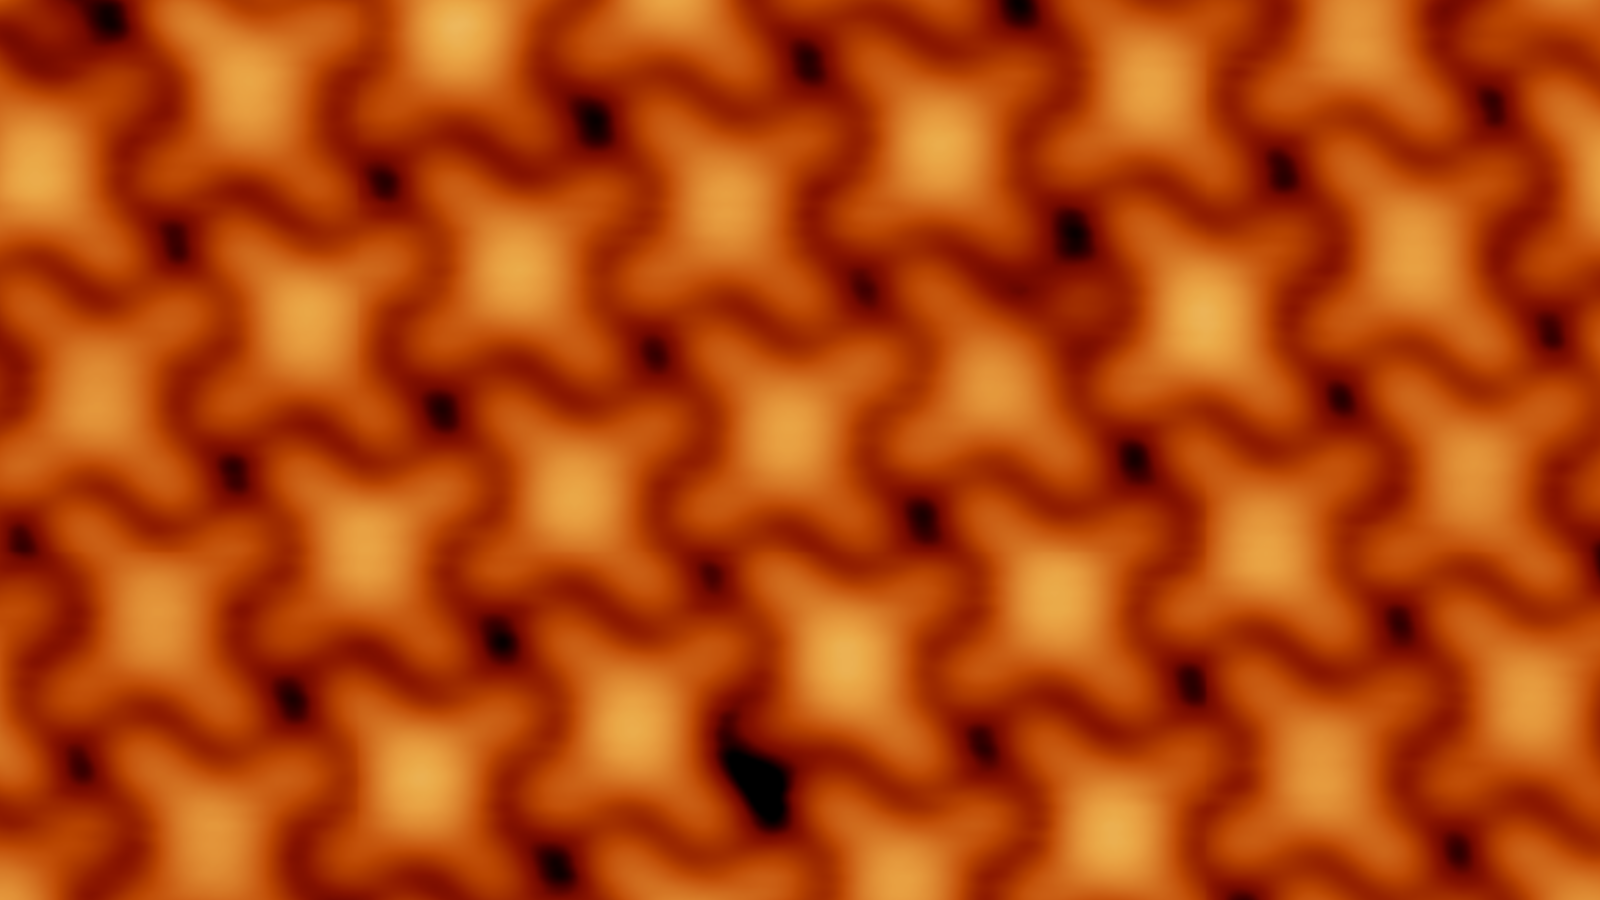
\includegraphics[width=0.7\textwidth]{./images/paper/pyrene/figure-3a}
		\label{fig:pyrene-fig3a}
	}
	\subfigure[]{
		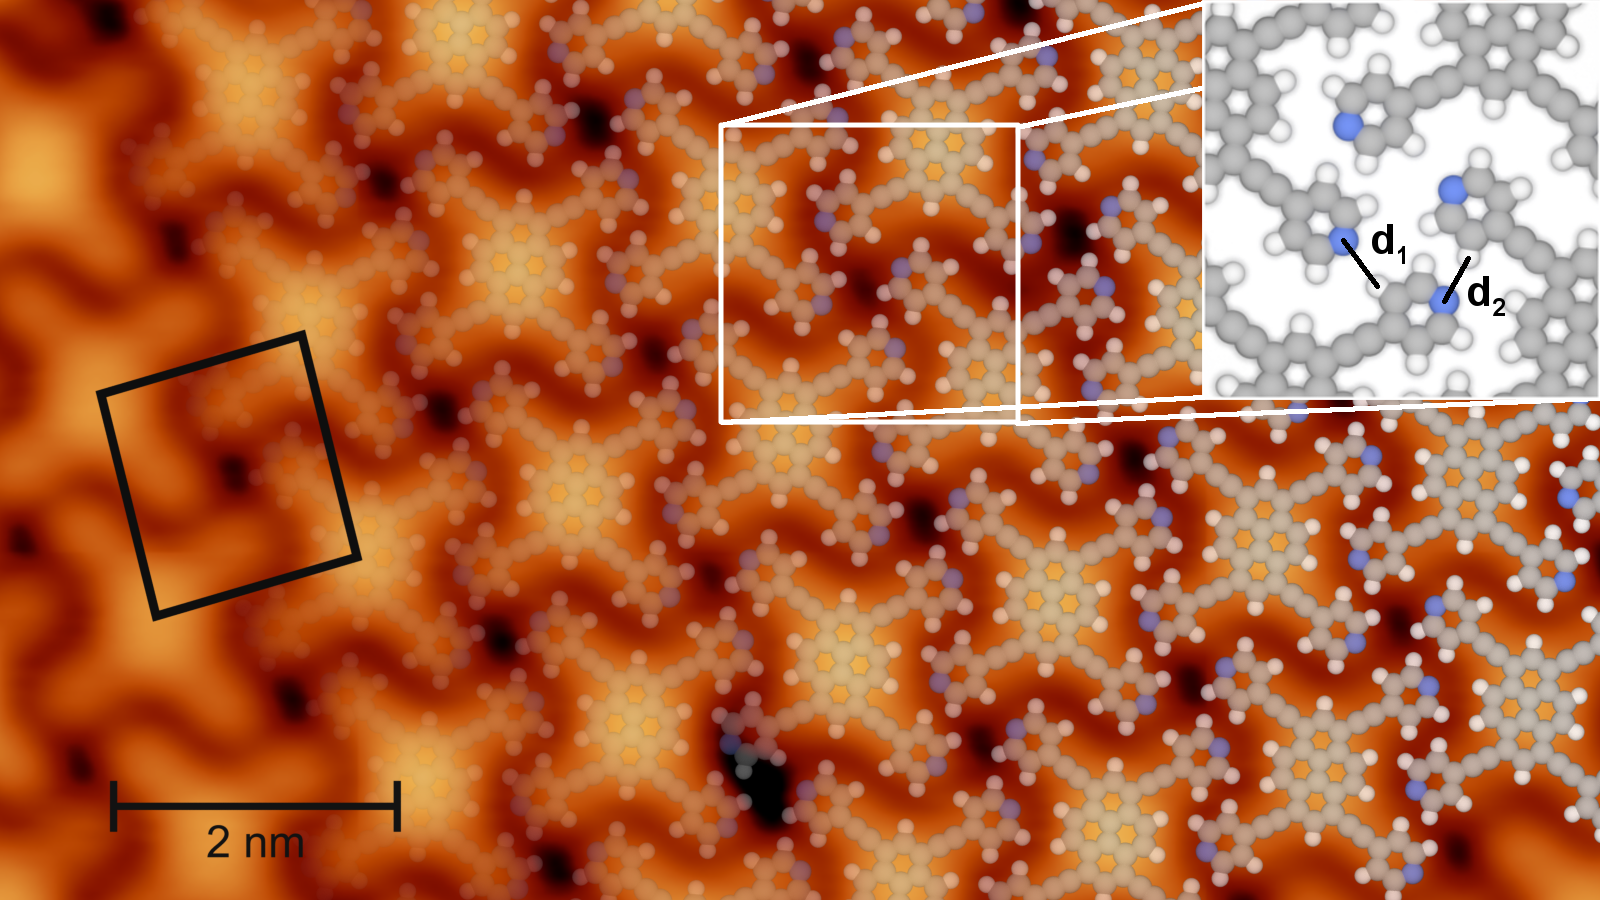
\includegraphics[width=0.7\textwidth]{./images/paper/pyrene/figure-3b}
		\label{fig:pyrene-fig3b}
	}
	\caption{STM topography of tetra-pyrene adsorbed on \textit{h}-BN/Cu(111). \subref{fig:pyrene-fig3a} Hexagonal moir\'e superstructure visible as bright protrusions. \subref{fig:pyrene-fig3b} After RT deposition the molecules assemble in dense packed islands in a square unit cell (black square). Molecular model superimposed. Inset (\SI{2}{\nano \meter} $\times$ \SI{2}{\nano \meter}) shows inter molecular distances $d_1$ and $d_2$. 
		Imaging parameters: 
		\subref{fig:pyrene-fig3a} \SI{2}{\volt}, \SI{0.1}{\nano \ampere}, \textcolor{red}{Image width:} and 
		\subref{fig:pyrene-fig3b} \SI{0.1}{\volt}, \SI{0.2}{\nano \ampere}, \textcolor{red}{Image width:}
	}
	\label{fig:pyrene-fig3}
\end{figure}

$d_1$ and $d_2$ equal \SI{0.288}{\nano \meter} and \SI{0.254}{\nano \meter} respectively and are both comparable to experimental\cite[5]{Kaposi_Supramolecular_2016} (\SI{0.27 \pm 0.05}{\nano \meter}) and theoretical\cite[5]{Arras_Nature_2012} (\SI{0.27}{\nano \meter}) results (\textcolor{red}{\textbf{find more of those!}}). Though hard to address quantitatively in STM a small tilt of the pyridil termini is likely present to compensate for the close proximity of the H-terminated pyridil rings and is observed as minor contrast differences within the four legs of the molecule. This tilt may enable interactions between the N terminated pyridil group and the pi system of the neighboring pyridil group, giving rise to an additional binding component beside a strict N-H hydrogen bonding.

%%
In addition to the topographic structure, STS reveals the electronic structure of the assembly. All spectra shown in \autoref{fig:pyrene-fig4b} are taken on the center of a molecule. Colored spectra and points (\autoref{fig:pyrene-fig4a}) indicate their distance to the \textit{h}-BN pore that is recognized as bright protrusion in \autoref{fig:pyrene-fig4b}. The darker the color of the points/spectra the larger the lateral distance to the pore. Molecular orbital energies are indicated by yellow (HOMO) and blue (LUMO) boxes. A blue arrow illustrates the electronic gap between both. Spectra have been fitted with a gauss function after background subtraction to determine the corresponding electronic states. The energy onset of HOMO is located between \SIrange{-1541}{-1583}{\milli \volt} with a dependence on the position within the moir\'e unit cell of 42 mV. The LUMO emerges at 
\SIrange{886}{1198}{\milli \volt}
%(886 ± 1) – (1198 ± 1) mV, 
with a notable shift of \SI{312}{\milli \volt} that compares well to the reported change in work function of the \textit{h}-BN/Cu(111) substrate.\cite{Sushobhan_Control_2014,Liu_Interplay_2015,Schulz_Templated_2013,urgel_controlling_2015} This is in good agreement with literature reporting different level alignment for occupied and unoccupied molecular orbitals where the larger shift of the LUMO mainly determines the electronic gap. It is smaller close to the pores.\cite{Kumar_Molecular_2017} The large gap between HOMO and LUMO (\SI{2.56}{\eV}) benefits molecular orbital resolution (Figure S4) and indicates efficient decoupling from the metallic substrate due to the insulating \textit{h}-BN spacer. 

\begin{figure}[] \centering
	\subfigure[]{
	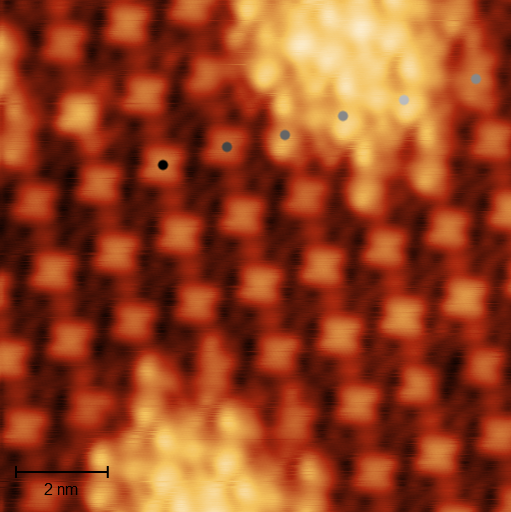
\includegraphics[height=5cm]{./images/paper/pyrene/figure-4b}
	\label{fig:pyrene-fig4b}
	}
	\subfigure[]{
		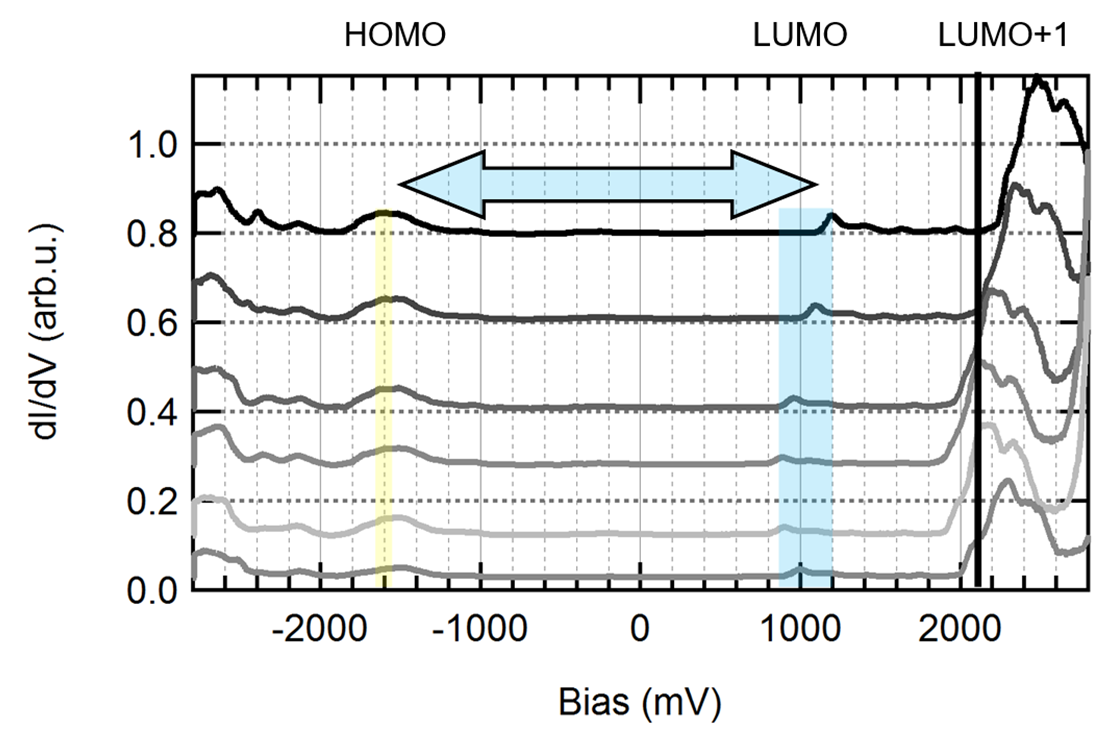
\includegraphics[height=5cm]{./images/paper/pyrene/figure-4a}
		\label{fig:pyrene-fig4a}
	}
	\caption{Spatial variation of molecular energy states within the moir\'e of tetra-pyrene. \subref{fig:pyrene-fig4a} STS on varying positions within moir\'e unit cell. HOMO and LUMO are indicated by yellow and blue boxes connected by an arrow indicating the electronic gap. A black vertical line is drawn close to the onset of LUMO+1 states at which energy the topography in \subref{fig:pyrene-fig4b}) was recorded. \subref{fig:pyrene-fig4b} STM topography where colored points indicate positions of spectra shown in \subref{fig:pyrene-fig4a}. Imaging parameter: \SI{11.07}{\nano \meter}, \SI{2.05}{\volt}, \SI{0.8}{\nano \ampere}}
	\label{fig:pyrene-fig4}
\end{figure}

In addition to the topographic structure, STS reveals the electronic structure of the assembly. All spectra shown in \autoref{fig:pyrene-fig4a} are taken on the center of a molecule. Colored spectra and points (\autoref{fig:pyrene-fig4b}) indicate their distance to the \textit{h}-BN pore that is recognized as bright protrusion in \autoref{fig:pyrene-fig4b}. The darker the color of the points/spectra the larger the lateral distance to the pore. Molecular orbital energies are indicated by yellow (HOMO) and blue (LUMO) boxes. A blue arrow illustrates the electronic gap between both. Spectra have been fitted with a gauss function after background subtraction to determine the corresponding electronic states. The energy onset of HOMO is located between \SIrange{-1541}{-1583}{\milli \volt} with a dependence on the position within the moir\'e unit cell of 42 mV. The LUMO emerges at \SIrange{886}{1198}{\milli \volt}, with a notable shift of \SI{312}{\milli \volt} that compares well to the reported change in work function of the \textit{h}-BN/Cu(111) substrate.\cite{Sushobhan_Control_2014,Liu_Interplay_2015,Schulz_Templated_2013,urgel_controlling_2015} This is in good agreement with literature reporting different level alignment for occupied and unoccupied molecular orbitals where the larger shift of the LUMO mainly determines the electronic gap. It is smaller close to the pores.\cite{Kumar_Molecular_2017} The large gap between HOMO and LUMO (\SI{2.56}{\eV}) benefits molecular orbital resolution (Figure S4) and indicates efficient decoupling from the metallic substrate due to the insulating \textit{h}-BN spacer. 

\begin{figure}[] \centering
	\subfigure[]{
		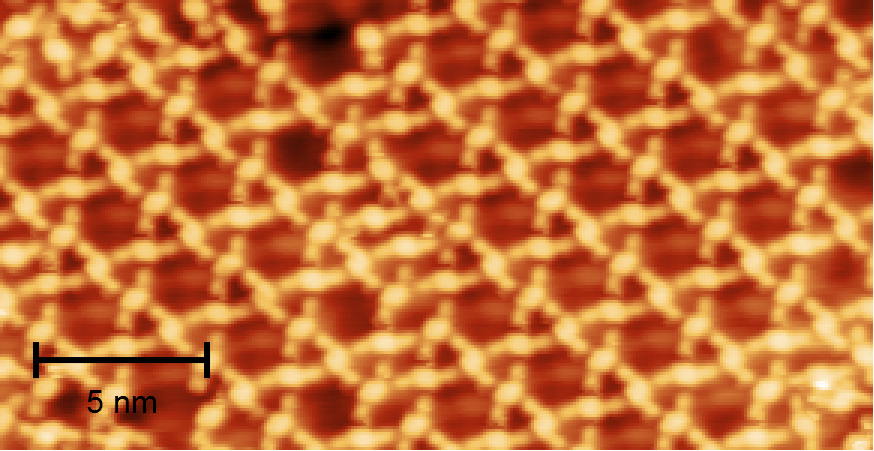
\includegraphics[width=0.7\textwidth]{./images/paper/pyrene/figure-5a}
		\label{fig:pyrene-fig5a}
	}
	\subfigure[]{
		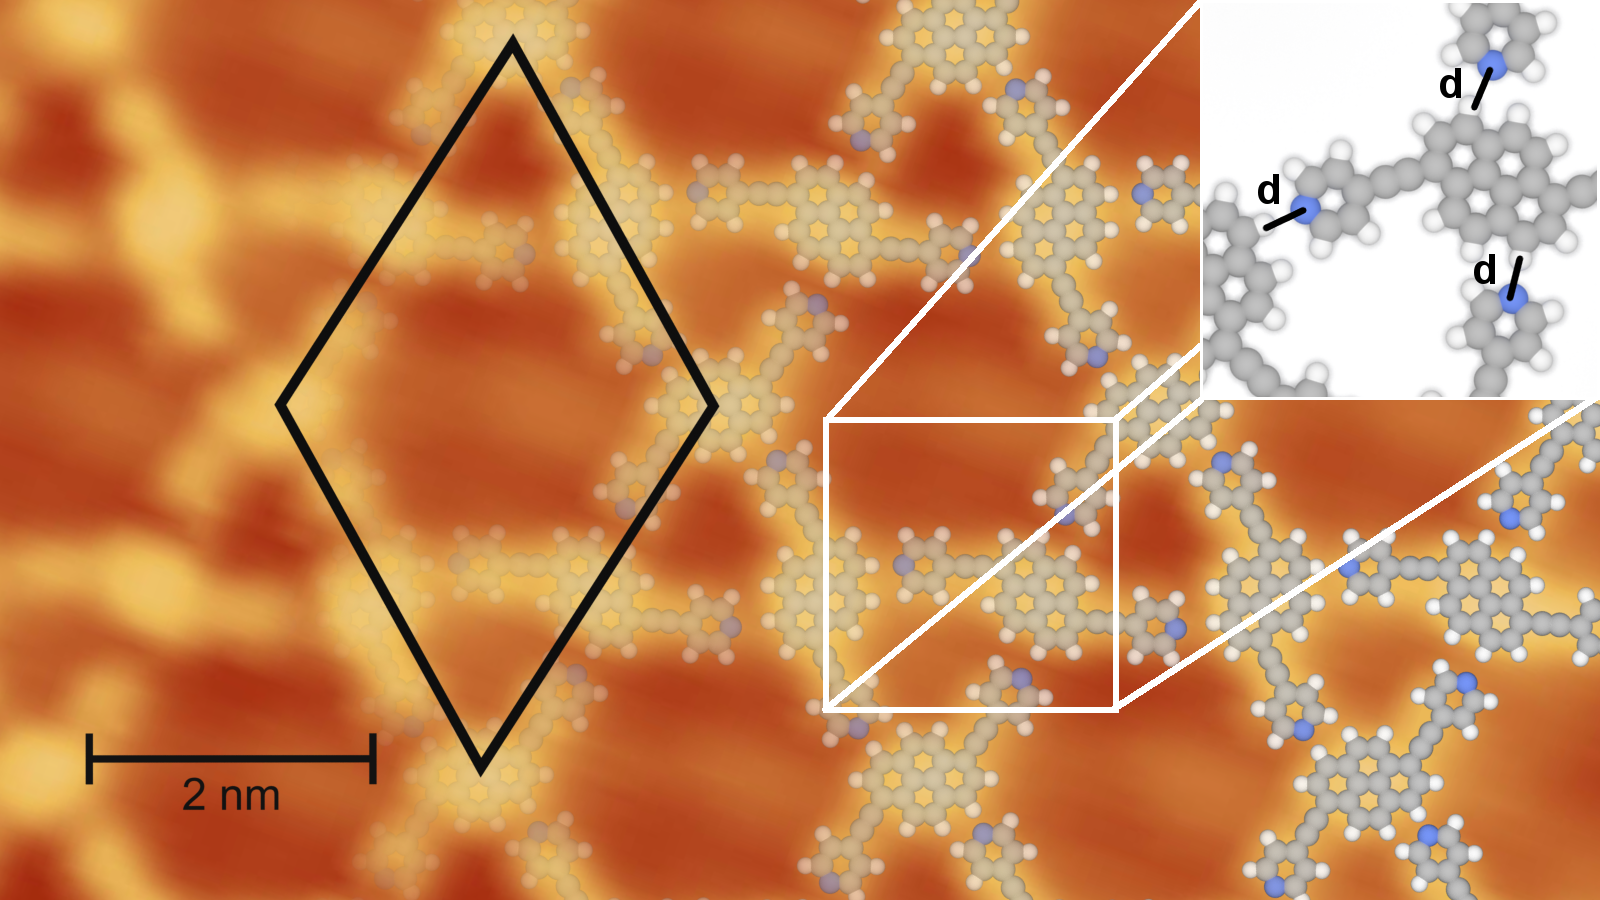
\includegraphics[width=0.7\textwidth]{./images/paper/pyrene/figure-5b}
		\label{fig:pyrene-fig5b}
	}
	\caption{Self-assembly of trans-pyrene on \textit{h}-BN/Cu(111). \subref{fig:pyrene-fig5a} STM topography of two homo-chiral domains with minor lateral offset to each other resulting in a narrow transition region between both. \subref{fig:pyrene-fig5b} Enlarged view on one domain with overlaid models and unit cell (black rhomb). Pyridil-pyrene core connections assemble open porous networks of hexagons and triangles (kagom\'e lattice) with well-defined binding distances $d$ (black lines in inset). Image parameters: \SI{1}{\volt}, \SI{0.1}{\nano \ampere}, \textcolor{red}{Image width:\subref{fig:pyrene-fig5a}, \subref{fig:pyrene-fig5b}}}
	\label{fig:pyrene-fig5}
\end{figure}

Reducing the number of substituents by depositing trans-pyrene onto the \textit{h}-BN/Cu(111) surface results in a drastic change in assembly. Now the molecules form open porous networks with a kagom\'e pattern (citation) as shown in \autoref{fig:pyrene-fig5}. The pro-chiral character of the molecule directly translates to the on surface assembly. A result is the formation of mirror domains (Figure S9). Each of the two consist of molecules with the same chirality (homo-chiral) while no domains with mixed chirality (hetero-chiral) are observed. Although a major surface area is covered by this regular pattern, homo-chiral domains are connected by narrow intermediate regions to compensate a lateral lattice offset. The connecting region between two domains with opposite chirality is usually larger. The unit cell of the kagom\'e pattern is ?rhombic? with (3.04 x 2.93) nm long unit cell vectors and holds three molecules. The hexagonal pores feature an edge length of about 1 nm. Although not every part of the surface was regularly covered with kagom\'e patterns of either chirality, the binding motif is controlled by N-H interactions between the nitrogen in the pyridil legs and the hydrogen terminated pyrene-core of their nearest neighbor. The distance d = (0.20 ± 0.02) nm (black lines in inset of \autoref{fig:pyrene-fig5}) is smaller compared to the on reported in the dense packed assembly of tetra-pyrene and compares (how) to some literature values … … (\textbf{citation!}). The shortened binding distance builds up stress in the assembly, a reason for the limited domain size of the assembly. For the distance given above, the molecules are assumed to lie flat on the surface – including the pyridil rings. A way to release some of the adlayer stress is to increase the tilt or rotation angle of the pyridil group, both increasing the binding distance.


\begin{figure}[] \centering
	\subfigure[]{
		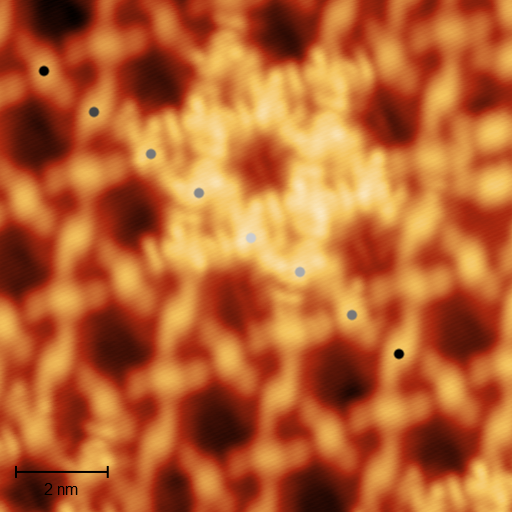
\includegraphics[height=5cm]{./images/paper/pyrene/figure-6b}
		\label{fig:pyrene-fig6b}
	}
	\subfigure[]{
		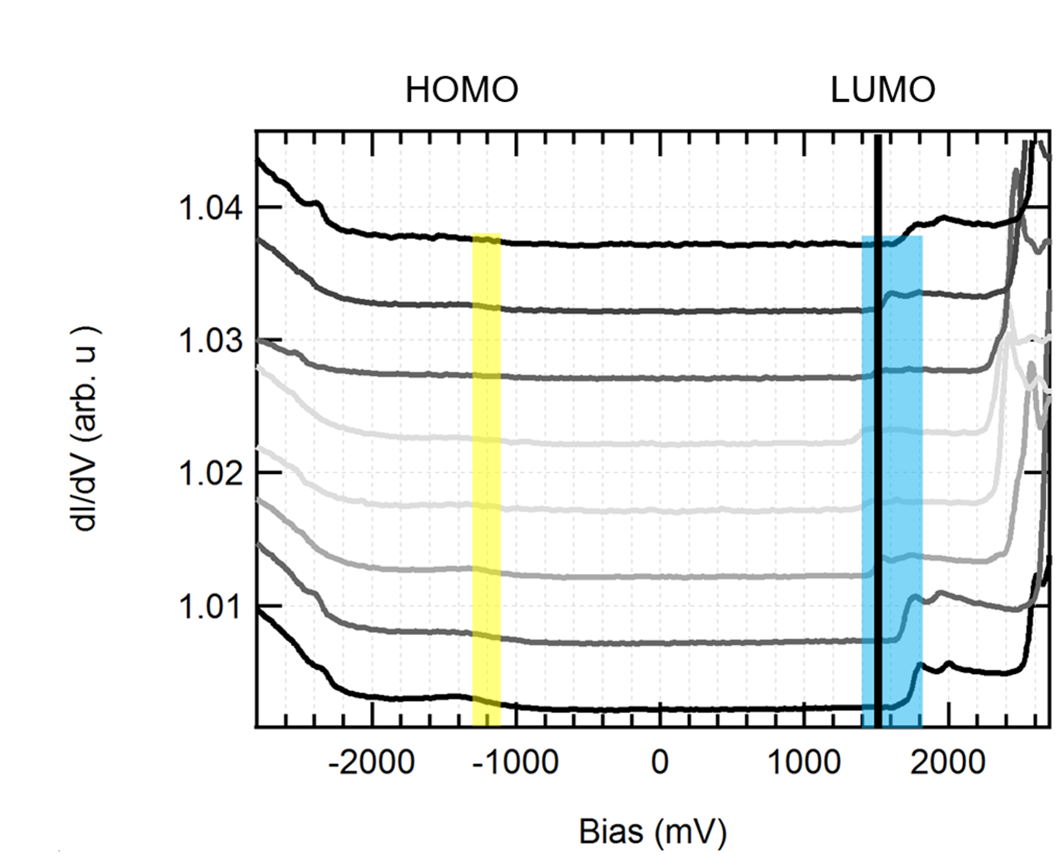
\includegraphics[height=5cm]{./images/paper/pyrene/figure-6a}
		\label{fig:pyrene-fig6a}
	}
	
	\caption{Spatial variation of the molecular states within the kagom\'e lattice formed by trans-pyrene on \textit{h}-BN/Cu(111). \subref{fig:pyrene-fig5a} Position and shift of HOMO (yellow) and LUMO (blue). \subref{fig:pyrene-fig5b} STM topography of a region where spectra across a moir\'e pore are taken. Colored points indicate the distance to the pores’ center. Imaging bias voltage is indicated in \subref{fig:pyrene-fig5a} by a black vertical line. Imaging parameter: \SI{11.07}{\nano \meter}, \SI{1.6}{\volt}, \SI{0.2}{\nano \ampere}
	}
	\label{fig:pyrene-fig6}
\end{figure}

To investigate the influence of the number of substituents on the electronic structure, STS is a capable technique. For trans-pyrene the HOMO in located between 
%(-1368 ± 4) and (-1490 ± 3) mV 
\SI{-1368}{\milli \volt} \& \SI{-1409}{\milli \volt}
and a LUMO between 
%(1478 ± 1) and (1816 ± 1) mV.
\SI{1478}{\milli \volt} \& \SI{1816}{\milli \volt}
 The resulting average gap between HOMO and LUMO is \SI{3051}{\milli \volt}. Molecular orbitals on pore positions of the \textit{h}-BN layer are again shifted to lower energies as compared to molecular orbitals on wire positions. The shift in LUMO energy (\SI{338}{\milli \volt}) is larger than the shift in the occupied states (\SI{122}{\milli \volt}). 
ST spectra show a large bandgap in between the HOMO and LUMO (\SI{3.05}{\eV}), which matches DFT results (\SI{2.95}{\eV}) very well. Compared to the electronic gap of the tetra-substituted species, the gap of the bis-substituted trans-pyrene is \SI{378}{\milli \volt} larger, following the trend of increasing electronic gaps with decreasing number of functional groups reflected in the DFT calculations.

\begin{figure}[] \centering
	\subfigure[]{
		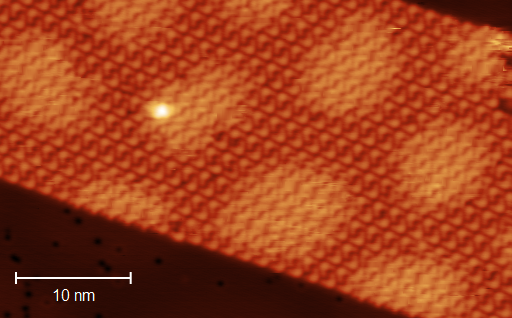
\includegraphics[width=0.7\textwidth]{./images/paper/pyrene/figure-7a}
		\label{fig:pyrene-fig7a}
	}
	\subfigure[]{
		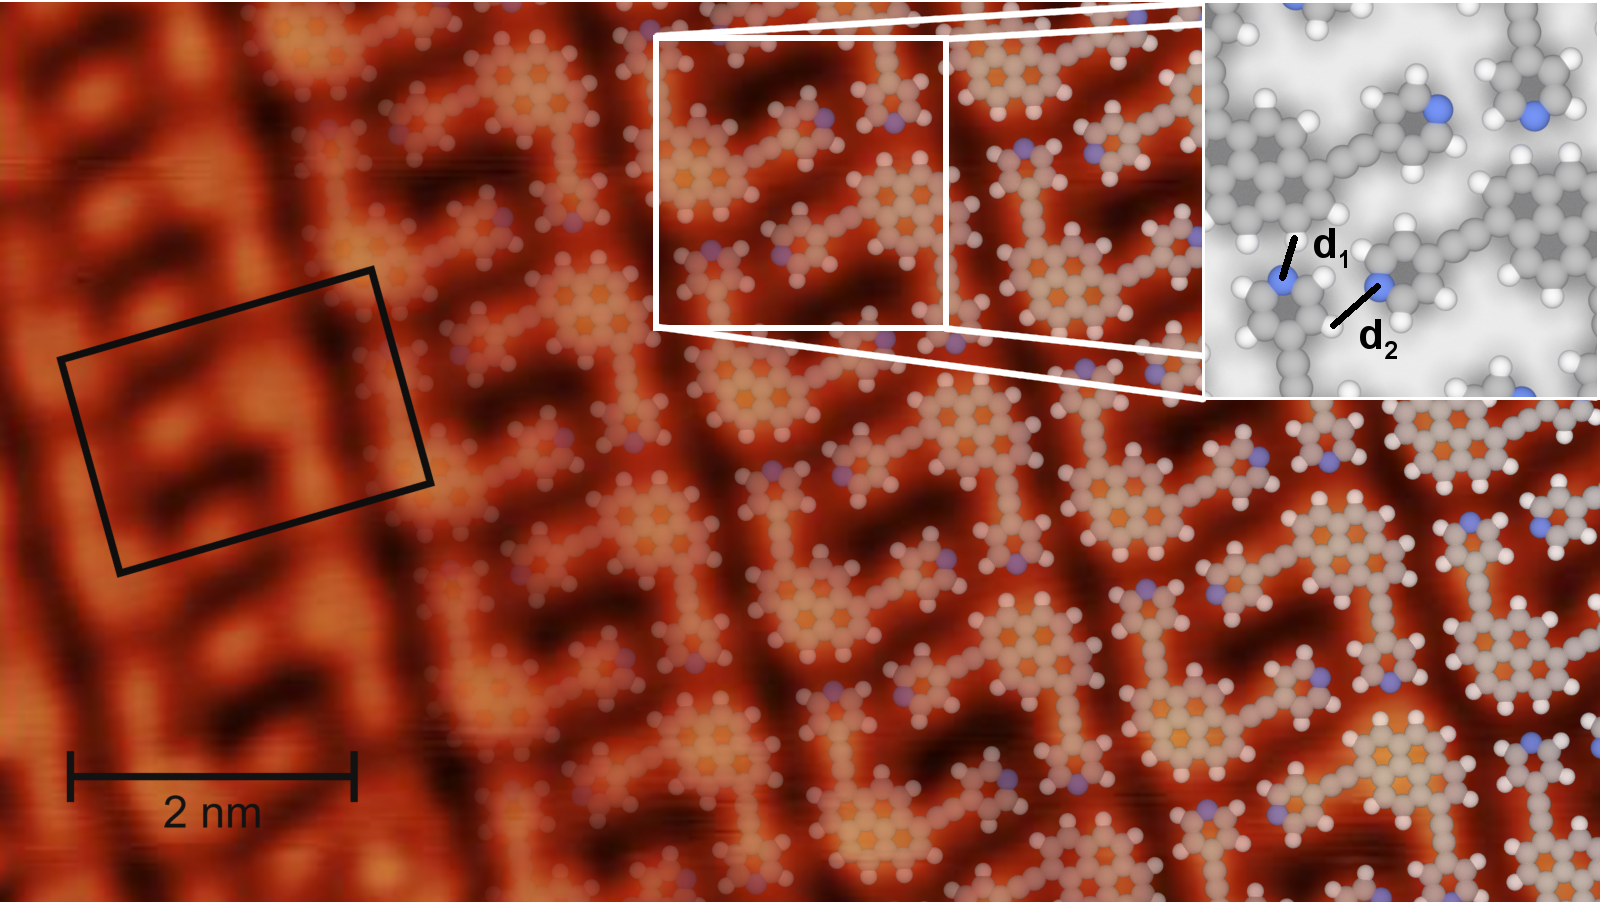
\includegraphics[width=0.7\textwidth]{./images/paper/pyrene/figure-7b}
		\label{fig:pyrene-fig7b}
	}
	\caption{Molecular self-assembly upon adsorption of cis-pyrene on \textit{h}-BN/Cu(111). White arrows indicate the preferred growth direction. \subref{fig:pyrene-fig7a} The electronic corrugation of the \textit{h}-BN (moir\'e) is visible as protrusions in LT-STM. \subref{fig:pyrene-fig7b} Overlaid molecular models of the binding motif. Unit cell is sketched as black rectangle. Enlarged inset depicts the binding distances ($d_1/d_2$) within this motif. Image parameters: \subref{fig:pyrene-fig7a} \SI{1.38}{\volt}, \SI{0.02}{\nano \ampere}, \textcolor{red}{Image width:}, \subref{fig:pyrene-fig7b} \SI{1}{\volt}, \SI{0.27}{\nano \ampere}, \textcolor{red}{Image width:}.
	}
	\label{fig:pyrene-fig7}
\end{figure}

To rule out a drastic influence of the assembly on the electronic structure we deposited cis- functionalized pyrenes. These molecules form extended, well ordered, dense packed islands, composed of rows along a preferred growth direction (compare island perimeter and white arrow in \autoref{fig:pyrene-fig7a}). Every row is composed of molecules that interconnect like tooth in a zip fastener. Molecules on one side of the fastener show the same orientation where those in the other half are rotated by \SI{180}{\degree}. The interconnection between both in shown in the inset of \autoref{fig:pyrene-fig7b} and stabilized by two bonds along $d_1$ and $d_2$. The two sides of the zip are bound via N-H binding along $d_2$ (\SI{0.298 \pm 0.01}{\nano \meter}). Within each side of the zip connection a bond between the nitrogen terminated leg and hydrogen terminated core of the trans-pyrene molecules guides chain formation along $d_1$ (\SI{0.284 \pm 0.01}{\nano \meter}, resulting in the above mentioned preferred growth direction. Stability within an island (i.e. perpendicular to the indicated growth direction) is maintained through vdW interactions of a molecules’ passivated pyrene-core to its neighbors’ with an average distance of \SI{0.26 \pm 0.05}{\nano \meter}. A unit cell within the island (black rectangle in \autoref{fig:pyrene-fig7b}, \SI{2.27}{\nano \meter} $\times$ \SI{1.57}{\nano \meter}) is made up of 2 molecules. Binding distances compare well to those present for tetra-pyrene on \textit{h}-BN where extended islands are found, too. The binding distance is comparable to those on Ag(111) as well. \cite{Kaposi_Supramolecular_2016}
The electronic structure of cis-pyrene is studied in STS. Cis-pyrene adsorbed on \textit{h}-BN (\autoref{fig:pyrene-fig8}) show a HOMO located between \SI{-1606}{\milli \volt} \& \SI{-1689}{\milli \volt} and a LUMO between \SI{1242}{\milli \volt} \& \SI{1602}{\milli \volt}. This results in an average gap between HOMO and LUMO of \SI{3.11}{\volt}. Again the shift of the LUMO is more pronounced (\SI{375}{\milli \volt}) than for the HOMO (\SI{84}{\milli \volt}). 

\begin{figure}[] \centering
	\subfigure[]{
		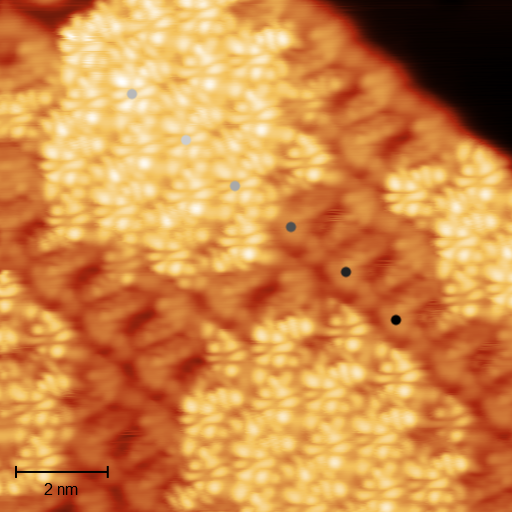
\includegraphics[height=5cm]{./images/paper/pyrene/figure-8b}
		\label{fig:pyrene-fig8b}
	}
	\subfigure[]{
		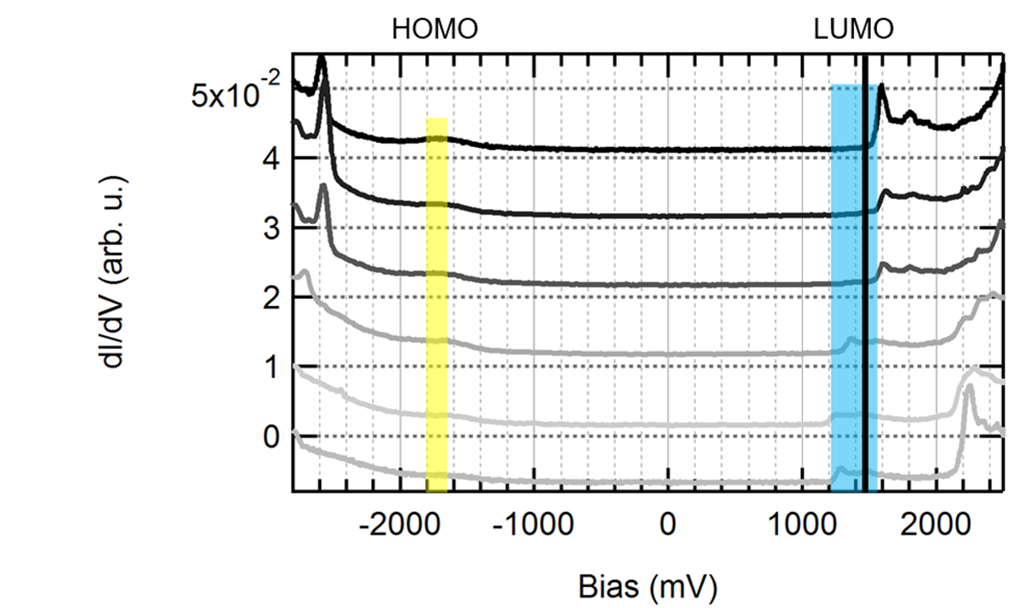
\includegraphics[height=5cm]{./images/paper/pyrene/figure-8a}
		\label{fig:pyrene-fig8a}
	}
	\caption{\subref{fig:pyrene-fig8a} STS measurements on cis-pyrene on \textit{h}-BN/Cu(111) across a moir\'e unit cell. HOMO (yellow), LUMO (blue) and the bias voltage used in \subref{fig:pyrene-fig8b} (black vertical line). \subref{fig:pyrene-fig8b} STM topography showing moir\'e pores with colored points indicating the positions of spectra in \subref{fig:pyrene-fig8a}. Imaging parameter: \SI{11.07}{\nano \meter}, \SI{1.5}{\volt}, \SI{0.1}{\nano \ampere}.
	}
	\label{fig:pyrene-fig8}
\end{figure}

The effect of increasing number of substituents and the accompanied change in self–assembly affects its electronic structure. For the dense packed motifs (trans- \& cis-pyrene) the band gap increases with decreasing number of substituents (2.56 \& 3.11 eV). Changing the surface tessellation while maintaining the number of substituents (trans- \& cis-pyrene) results in almost no change (3.05 \& 3.11 eV). This indicates that changing the number of substituents has a larger impact on the electronic gap than an increased screening introduced by a larger number of nearest neighbors.

\begin{figure}[] \centering
	\subfigure[]{
		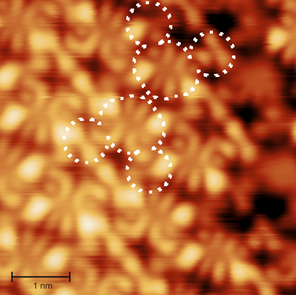
\includegraphics[height=5cm]{./images/paper/pyrene/figure-9a}
		\label{fig:pyrene-fig9a}
	}
	\subfigure[]{
		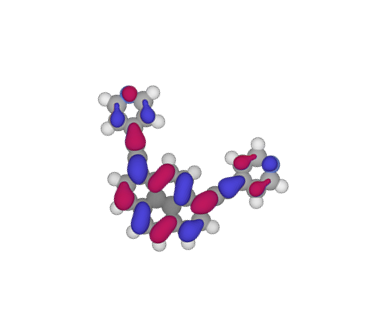
\includegraphics[height=5cm]{./images/paper/pyrene/figure-9b}
		\label{fig:pyrene-fig9b}
	}
	\caption{Structure of unoccupied frontier orbital. \subref{fig:pyrene-fig9a} STM image recorded close to the onset of the LUMO energy. White dashed lines indicate the perimeter of two molecules. Imaging parameters: \SI{1.5}{\volt}, \SI{0.27}{\nano \ampere}, \textcolor{red}{Image width:}. \subref{fig:pyrene-fig9b} DFT-calculation.
	}
	\label{fig:pyrene-fig9}
\end{figure}

The previous STS measurements show the \textit{h}-BN’s ability to effectively decouple the electronic systems of molecules and metallic substrate. This can be used to image the shape of frontier orbitals directly in STM. Recording STM topography images close to the onset of the LUMO frontier orbital resolution is achieved (\autoref{fig:pyrene-fig8b}). A closer look (\autoref{fig:pyrene-fig9a}) reveals the real space distribution. For better visibility two molecules are outlined in white. One can recognize four central lobes along the short axes of the pyrene core and three dots on the leg positions. Comparing the contrast of these features with DFT calculation suggests a tunneling process where tunneling is indeed mediated by the first unoccupied molecular orbital as calculated by DFT in gas phase (\autoref{fig:pyrene-fig9b}).


\begin{figure}[] \centering
	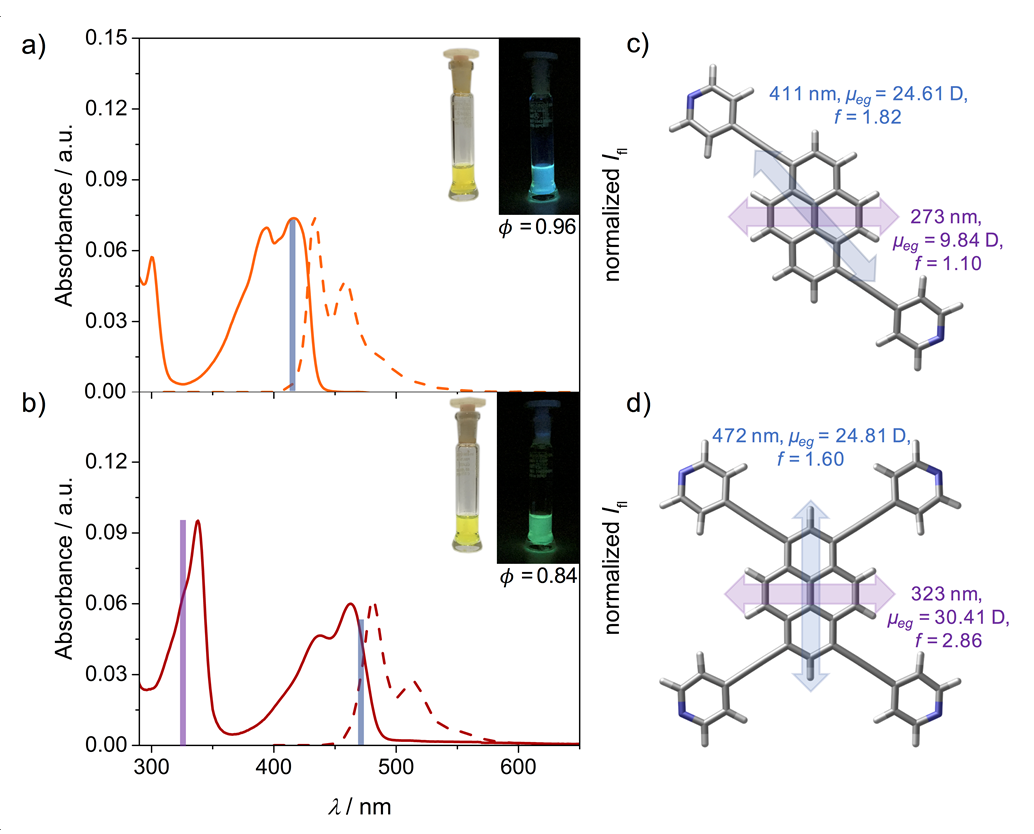
\includegraphics[width=0.7\textwidth]{./images/paper/pyrene/figure-10}
	\caption{a, b) UV/Vis absorption (solid line) and emission spectra (dotted line) of trans-pyrene (a, orange line) and tetra-pyrene (b, red line) in toluene (c = \SI{e-6}{\mole}) at room temperature. Insets: photographs of toluene solutions under daylight and upon irradiation with a hand-held UV lamp ($\lambda_{ex} = \SI{365}{\nano \meter}$). c, d) Calculated transitions (blue and purple lines), transition dipole moments ($\mu_{eg}$), and oscillator strengths ($f$) as determined by TD-DFT (CAM-B3LYP, 6-31G*).}
	\label{fig:pyrene-fig10}
\end{figure}


The photophysical properties, in diluted toluene solutions, of trans- \& tetra-pyrene are displayed in \autoref{fig:pyrene-fig10}(a) and (b). The absorption spectrum of trans-pyrene shows two main absorption peaks at \SI{416}{\nano \meter} and \SI{394}{\nano \meter}, with another lower absorption band located at higher energy (300 nm). Exciting the low energy absorption peak leads to strong emission at \SI{433}{\nano \meter} and \SI{458}{\nano \meter}, with a quantum yield of \SI{96}{\percent} (determined using Coumarin 153 in ethanol solution as reference). As expected, the tetra-substituted pyrene shows absorption peaks that are bathochromically shifted towards lower energies, with two main bands observed at \SI{463}{\nano \meter} and \SI{438}{\nano \meter} nm and a higher energy, more allowed, peak at \SI{338}{\nano \meter}. Excitation of tetra-pyrene in the lowest energy bands also leads to strong emission, found at \SI{481}{\nano \meter} and \SI{513}{\nano \meter}, with a quantum yield of \SI{84}{\percent}. The same optical transitions seem to be involved in both the absorption and emission processes, as confirmed by a good mirror symmetry of the fluorescent spectra compared to lowest energy absorption transitions. Moreover, the small Stokes shifts (\SI{17}{\nano \meter} and \SI{18}{\nano \meter} for trans- and tetra-pyrene, respectively) are due to the similar geometric structures of the ground and excited states, while the matching excitation and absorption spectra point to an efficient radiative deactivation of the excited state (Figure S11).\cite{Diring_Luminescent_2009}
In relation to the above experimental results, we performed time-dependent density function method (TD-DFT) calculations (CAM-B3LYP/6-31G**, toluene CPCM solvation), \cite{Kurata_donor_2017, Ji_Electron_2015} summarized in Figures 10c, d and S2. The main transitions for trans-pyrene seem to originate from the $H \rightarrow L$ (estimated at $\lambda = \SI{411}{\nano\meter}, f = 1.82$) and $H-1 \rightarrow L / H \rightarrow L+2 transitions (estimated at \lambda = \SI{273}{\nano \meter}, f = 1.10$), with the transition dipole moments aligned along the 1- and 6-positions (towards the pyridylethynyl termini) and the short molecular axes of the central pyrene core. On the other hand, tetra-pyrenes transition dipole moments are aligned along the long and short molecular axes of the pyrene core, with the two main transitions having $H \rightarrow L$ (estimated at $\lambda = \SI{472}{\nano \meter}, f = 1.60$) and $H-1 \rightarrow L / H \rightarrow L+1$ (estimated at $\lambda = \SI{323}{\nano \meter}, f = 2.84$) contributions.

\subsection{Summary / Discussion}
Here we investigated a benchmark system for unperturbed pyridil functionalized pyrenes on an inert substrate in UHV. Bis- \& Tetra-pyridin-4-ylethynyl functionalized pyrene molecules are investigated with STM/STS on a \textit{h}-BN/Cu(111) surface as well as by means of UV/Vis spectroscopy in solution and ab initio calculations in gas-phase.
Reminiscent of adsorption on Ag(111)(citation) substrates the pyrene core adsorbs flat on the substrate. The different assemblies on \textit{h}-BN/Cu(111) are a direct result of the stabilizing binding motifs that can be tuned by the number \& position of functional groups. Depended on these design considerations open porous networks and dense packed assemblies are formed on the surface.
TETRA: For tetra-pyrene the dense packed assembly is a result of an interaction solely between pyridil legs. A rotation of the pyridil ring makes its delocalized electronic pi system accessible for the nitrogen terminated pyridil ring of  its neighbors.
TRANS: For trans-pyrene the position of the pyridil legs cause a kagom\'e network solely stabilized by connections between pyridil rings and pyrene cores, constructing a binding to stabilize open, hexagonal pores. Only the pyrene core is assumed to adsorb flat on the surface. The shorter binding distance introduces stress in the adlayer, compensated by the pyridil leg being rotated around the C-C bond and therefor increasing the binding distance. The molecules’ pro-chiral property transfers to the assembly and forms two homo-chiral mirror domains. 
CIS: In contrast to the adsorption on Ag(111), where dense packed structures are achieved only at higher coverages(citation), cis-pyrene on \textit{h}-BN/Cu(111) develops extended islands. The reported (citation) Ag-adatom mediated head-to-head coupling motif is not observed here, but only on the bare metal substrate. This is because in contrast to Ag(111) there are no metal ad-atoms available on \textit{h}-BN. The binding motif within the assembly shows both, interaction between rotated legs, and towards flat adsorbed pyrene cores.
STS shows prominent HOMO/LUMO features that are a result of the efficient decoupling from the metallic substrate via the \textit{h}-BN layer. These shift in the same direction but by different amount related to the molecules' position in the moir\'e. The electronic gap is predominantly determined by the larger shift of unoccupied states which are closer to fermi energy on moir\'e pore sites. Hence a smaller gap is created on pores while the gap is larger on wire sites, highlighting the use of \textit{h}-BN as a work function template for adsorbates.
While an increasing number of functional groups reduces the electronic gap in accordance with other reports on similar systems (citation), the assemblies’ effect on the band gap is investigated by bis-substituted pyrene derivatives (trans- \& cis-pyrene). Here the number of substituents remains the same and the assemblies’ effect on the band gap can be investigated. A minor change between open-porous (trans-pyrene, \SI{3.05}{\eV}) and dense packed (cis-pyrene, \SI{3.11}{\eV}) assemblies (\SI{60}{\milli \eV}) can be linked to the increased screening for dense packed assemblies (citation for similar systems!).
Since optical properties are a directly linked to the band gap UV/Vis adsorption measurements are used as complementary technique and reveals peaks at 416/394 nm (trans) and \SI{463}{\nano \meter}/\SI{438}{\nano \meter} (tetra). Emission spectra show distinct features at \SI{433}{\nano \meter}/\SI{458}{\nano \meter}, \SI{96}{\percent}(trans) and \SI{481}{\nano \meter}/\SI{513}{\nano \meter}, \SI{84}{\percent} (tetra). These correlate well with TD-DFT calculations predicting $H \rightarrow L$ \& $H-1 \rightarrow L / H \rightarrow L+2$ (\SI{411}{\nano \meter} \& \SI{273}{\nano \meter} for trans-pyrene) and $H \rightarrow L \& H-1 \rightarrow L / H \rightarrow L+1$ (\SI{472}{\nano \meter} \& \SI{323}{\nano \meter} for tetra-pyrene) transitions. 
Ab initio calculations are in agreement with STS and UV/Vis measurements supporting electronically decoupled molecules as well for the \textit{h}-BN/Cu(111) surface in UHV as in solution. They also confirm the trend of increasing band gap with decreasing number of substituents as found in STS. 
[]
\subsection{Conclusion}
The novel, optically active bis- \& tetra-pyridin-4-ylethynyl functionalized pyrene molecule self-assembles on the isolating \textit{h}-BN/Cu(111) surface in networks on the nm scale that are stabilized by an attractive interaction of pyridil legs. While cis- \& tetra-functionalization results in close packed assemblies, trans-functionalization leads to open porous networks on \textit{h}-BN/Cu(111) that may be further investigated regarding their role as host for different molecules. The electronic gap is decreasing with increasing number of substituents. The electronically corrugated \textit{h}-BN/Cu(111) interface acts as work function template for the adsorbed molecules where the size of the gap is related to the adsorption site within the moir\'e. The optical properties of the molecules are addressed by means of UV-/Vis spectroscopy and show distinct fluorescence emission with high quantum yield that are applicable in a variety of devices and applications.